
%% bare_conf.tex
%% V1.3
%% 2007/01/11
%% by Michael Shel
%% See:
%% http://www.michaelshell.org/
%% for current contact information.
%%
%% This is a skeleton file demonstrating the use of IEEEtran.cls
%% (requires IEEEtran.cls version 1.7 or later) with an IEEE conference paper.
%%
%% Support sites:
%% http://www.michaelshell.org/tex/ieeetran/
%% http://www.ctan.org/tex-archive/macros/latex/contrib/IEEEtran/
%% and
%% http://www.ieee.org/

%%*************************************************************************
%% Legal Notice:
%% This code is offered as-is without any warranty either expressed or
%% implied; without even the implied warranty of MERCHANTABILITY or
%% FITNESS FOR A PARTICULAR PURPOSE! 
%% User assumes all risk.
%% In no event shall IEEE or any contributor to this code be liable for
%% any damages or losses, including, but not limited to, incidental,
%% consequential, or any other damages, resulting from the use or misuse
%% of any information contained here.
%%
%% All comments are the opinions of their respective authors and are not
%% necessarily endorsed by the IEEE.
%%
%% This work is distributed under the LaTeX Project Public License (LPPL)
%% ( http://www.latex-project.org/ ) version 1.3, and may be freely used,
%% distributed and modified. A copy of the LPPL, version 1.3, is included
%% in the base LaTeX documentation of all distributions of LaTeX released
%% 2003/12/01 or later.
%% Retain all contribution notices and credits.
%% ** Modified files should be clearly indicated as such, including  **
%% ** renaming them and changing author support contact information. **
%%
%% File list of work: IEEEtran.cls, IEEEtran_HOWTO.pdf, bare_adv.tex,
%%                    bare_conf.tex, bare_jrnl.tex, bare_jrnl_compsoc.tex
%%*************************************************************************

% *** Authors should verify (and, if needed, correct) their LaTeX system  ***
% *** with the testflow diagnostic prior to trusting their LaTeX platform ***
% *** with production work. IEEE's font choices can trigger bugs that do  ***
% *** not appear when using other class files.                            ***
% The testflow support page is at:
% http://www.michaelshell.org/tex/testflow/



% Note that the a4paper option is mainly intended so that authors in
% countries using A4 can easily print to A4 and see how their papers will
% look in print - the typesetting of the document will not typically be
% affected with changes in paper size (but the bottom and side margins will).
% Use the testflow package mentioned above to verify correct handling of
% both paper sizes by the user's LaTeX system.
%
% Also note that the "draftcls" or "draftclsnofoot", not "draft", option
% should be used if it is desired that the figures are to be displayed in
% draft mode.
%
\documentclass[10pt, conference, compsocconf]{IEEEtran}
% Add the compsocconf option for Computer Society conferences.
%
% If IEEEtran.cls has not been installed into the LaTeX system files,
% manually specify the path to it like:
% \documentclass[conference]{../sty/IEEEtran}

% Some very useful LaTeX packages include:
% (uncomment the ones you want to load)


% *** MISC UTILITY PACKAGES ***
%
%\usepackage{ifpdf}
% Heiko Oberdiek's ifpdf.sty is very useful if you need conditional
% compilation based on whether the output is pdf or dvi.
% usage:
% \ifpdf
%   % pdf code
% \else
%   % dvi code
% \fi
% The latest version of ifpdf.sty can be obtained from:
% http://www.ctan.org/tex-archive/macros/latex/contrib/oberdiek/
% Also, note that IEEEtran.cls V1.7 and later provides a builtin
% \ifCLASSINFOpdf conditional that works the same way.
% When switching from latex to pdflatex and vice-versa, the compiler may
% have to be run twice to clear warning/error messages.






% *** CITATION PACKAGES ***
%
%\usepackage{cite}
% cite.sty was written by Donald Arseneau
% V1.6 and later of IEEEtran pre-defines the format of the cite.sty package
% \cite{} output to follow that of IEEE. Loading the cite package will
% result in citation numbers being automatically sorted and properly
% "compressed/ranged". e.g., [1], [9], [2], [7], [5], [6] without using
% cite.sty will become [1], [2], [5]--[7], [9] using cite.sty. cite.sty's
% \cite will automatically add leading space, if needed. Use cite.sty's
% noadjust option (cite.sty V3.8 and later) if you want to turn this off.
% cite.sty is already installed on most LaTeX systems. Be sure and use
% version 4.0 (2003-05-27) and later if using hyperref.sty. cite.sty does
% not currently provide for hyperlinked citations.
% The latest version can be obtained at:
% http://www.ctan.org/tex-archive/macros/latex/contrib/cite/
% The documentation is contained in the cite.sty file itself.






% *** GRAPHICS RELATED PACKAGES ***
%
\ifCLASSINFOpdf
   \usepackage[pdftex]{graphicx}
  % declare the path(s) where your graphic files are
  \graphicspath{{../pdf/}{../jpeg/}}
  % and their extensions so you won't have to specify these with
  % every instance of \includegraphics
   \DeclareGraphicsExtensions{.pdf,.jpeg,.png}
\else
  % or other class option (dvipsone, dvipdf, if not using dvips). graphicx
  % will default to the driver specified in the system graphics.cfg if no
  % driver is specified.
  % \usepackage[dvips]{graphicx}
  % declare the path(s) where your graphic files are
  % \graphicspath{{../eps/}}
  % and their extensions so you won't have to specify these with
  % every instance of \includegraphics
  % \DeclareGraphicsExtensions{.eps}
\fi
% graphicx was written by David Carlisle and Sebastian Rahtz. It is
% required if you want graphics, photos, etc. graphicx.sty is already
% installed on most LaTeX systems. The latest version and documentation can
% be obtained at: 
% http://www.ctan.org/tex-archive/macros/latex/required/graphics/
% Another good source of documentation is "Using Imported Graphics in
% LaTeX2e" by Keith Reckdahl which can be found as epslatex.ps or
% epslatex.pdf at: http://www.ctan.org/tex-archive/info/
%
% latex, and pdflatex in dvi mode, support graphics in encapsulated
% postscript (.eps) format. pdflatex in pdf mode supports graphics
% in .pdf, .jpeg, .png and .mps (metapost) formats. Users should ensure
% that all non-photo figures use a vector format (.eps, .pdf, .mps) and
% not a bitmapped formats (.jpeg, .png). IEEE frowns on bitmapped formats
% which can result in "jaggedy"/blurry rendering of lines and letters as
% well as large increases in file sizes.
%
% You can find documentation about the pdfTeX application at:
% http://www.tug.org/applications/pdftex





% *** MATH PACKAGES ***
%
%\usepackage[cmex10]{amsmath}
% A popular package from the American Mathematical Society that provides
% many useful and powerful commands for dealing with mathematics. If using
% it, be sure to load this package with the cmex10 option to ensure that
% only type 1 fonts will utilized at all point sizes. Without this option,
% it is possible that some math symbols, particularly those within
% footnotes, will be rendered in bitmap form which will result in a
% document that can not be IEEE Xplore compliant!
%
% Also, note that the amsmath package sets \interdisplaylinepenalty to 10000
% thus preventing page breaks from occurring within multiline equations. Use:
%\interdisplaylinepenalty=2500
% after loading amsmath to restore such page breaks as IEEEtran.cls normally
% does. amsmath.sty is already installed on most LaTeX systems. The latest
% version and documentation can be obtained at:
% http://www.ctan.org/tex-archive/macros/latex/required/amslatex/math/





% *** SPECIALIZED LIST PACKAGES ***
%
\usepackage{algorithm,algorithmic}
% algorithmic.sty was written by Peter Williams and Rogerio Brito.
% This package provides an algorithmic environment fo describing algorithms.
% You can use the algorithmic environment in-text or within a figure
% environment to provide for a floating algorithm. Do NOT use the algorithm
% floating environment provided by algorithm.sty (by the same authors) or
% algorithm2e.sty (by Christophe Fiorio) as IEEE does not use dedicated
% algorithm float types and packages that provide these will not provide
% correct IEEE style captions. The latest version and documentation of
% algorithmic.sty can be obtained at:
% http://www.ctan.org/tex-archive/macros/latex/contrib/algorithms/
% There is also a support site at:
% http://algorithms.berlios.de/index.html
% Also of interest may be the (relatively newer and more customizable)
% algorithmicx.sty package by Szasz Janos:
% http://www.ctan.org/tex-archive/macros/latex/contrib/algorithmicx/




% *** ALIGNMENT PACKAGES ***
%
%\usepackage{array}
% Frank Mittelbach's and David Carlisle's array.sty patches and improves
% the standard LaTeX2e array and tabular environments to provide better
% appearance and additional user controls. As the default LaTeX2e table
% generation code is lacking to the point of almost being broken with
% respect to the quality of the end results, all users are strongly
% advised to use an enhanced (at the very least that provided by array.sty)
% set of table tools. array.sty is already installed on most systems. The
% latest version and documentation can be obtained at:
% http://www.ctan.org/tex-archive/macros/latex/required/tools/


%\usepackage{mdwmath}
%\usepackage{mdwtab}
% Also highly recommended is Mark Wooding's extremely powerful MDW tools,
% especially mdwmath.sty and mdwtab.sty which are used to format equations
% and tables, respectively. The MDWtools set is already installed on most
% LaTeX systems. The lastest version and documentation is available at:
% http://www.ctan.org/tex-archive/macros/latex/contrib/mdwtools/


% IEEEtran contains the IEEEeqnarray family of commands that can be used to
% generate multiline equations as well as matrices, tables, etc., of high
% quality.


%\usepackage{eqparbox}
% Also of notable interest is Scott Pakin's eqparbox package for creating
% (automatically sized) equal width boxes - aka "natural width parboxes".
% Available at:
% http://www.ctan.org/tex-archive/macros/latex/contrib/eqparbox/





% *** SUBFIGURE PACKAGES ***
%\usepackage[tight,footnotesize]{subfigure}
% subfigure.sty was written by Steven Douglas Cochran. This package makes it
% easy to put subfigures in your figures. e.g., "Figure 1a and 1b". For IEEE
% work, it is a good idea to load it with the tight package option to reduce
% the amount of white space around the subfigures. subfigure.sty is already
% installed on most LaTeX systems. The latest version and documentation can
% be obtained at:
% http://www.ctan.org/tex-archive/obsolete/macros/latex/contrib/subfigure/
% subfigure.sty has been superceeded by subfig.sty.



%\usepackage[caption=false]{caption}
%\usepackage[font=footnotesize]{subfig}
% subfig.sty, also written by Steven Douglas Cochran, is the modern
% replacement for subfigure.sty. However, subfig.sty requires and
% automatically loads Axel Sommerfeldt's caption.sty which will override
% IEEEtran.cls handling of captions and this will result in nonIEEE style
% figure/table captions. To prevent this problem, be sure and preload
% caption.sty with its "caption=false" package option. This is will preserve
% IEEEtran.cls handing of captions. Version 1.3 (2005/06/28) and later 
% (recommended due to many improvements over 1.2) of subfig.sty supports
% the caption=false option directly:
%\usepackage[caption=false,font=footnotesize]{subfig}
%
% The latest version and documentation can be obtained at:
% http://www.ctan.org/tex-archive/macros/latex/contrib/subfig/
% The latest version and documentation of caption.sty can be obtained at:
% http://www.ctan.org/tex-archive/macros/latex/contrib/caption/




% *** FLOAT PACKAGES ***
%
%\usepackage{fixltx2e}
% fixltx2e, the successor to the earlier fix2col.sty, was written by
% Frank Mittelbach and David Carlisle. This package corrects a few problems
% in the LaTeX2e kernel, the most notable of which is that in current
% LaTeX2e releases, the ordering of single and double column floats is not
% guaranteed to be preserved. Thus, an unpatched LaTeX2e can allow a
% single column figure to be placed prior to an earlier double column
% figure. The latest version and documentation can be found at:
% http://www.ctan.org/tex-archive/macros/latex/base/



%\usepackage{stfloats}
% stfloats.sty was written by Sigitas Tolusis. This package gives LaTeX2e
% the ability to do double column floats at the bottom of the page as well
% as the top. (e.g., "\begin{figure*}[!b]" is not normally possible in
% LaTeX2e). It also provides a command:
%\fnbelowfloat
% to enable the placement of footnotes below bottom floats (the standard
% LaTeX2e kernel puts them above bottom floats). This is an invasive package
% which rewrites many portions of the LaTeX2e float routines. It may not work
% with other packages that modify the LaTeX2e float routines. The latest
% version and documentation can be obtained at:
% http://www.ctan.org/tex-archive/macros/latex/contrib/sttools/
% Documentation is contained in the stfloats.sty comments as well as in the
% presfull.pdf file. Do not use the stfloats baselinefloat ability as IEEE
% does not allow \baselineskip to stretch. Authors submitting work to the
% IEEE should note that IEEE rarely uses double column equations and
% that authors should try to avoid such use. Do not be tempted to use the
% cuted.sty or midfloat.sty packages (also by Sigitas Tolusis) as IEEE does
% not format its papers in such ways.





% *** PDF, URL AND HYPERLINK PACKAGES ***
%
\usepackage{url}
% url.sty was written by Donald Arseneau. It provides better support for
% handling and breaking URLs. url.sty is already installed on most LaTeX
% systems. The latest version can be obtained at:
% http://www.ctan.org/tex-archive/macros/latex/contrib/misc/
% Read the url.sty source comments for usage information. Basically,
% \url{my_url_here}.





% *** Do not adjust lengths that control margins, column widths, etc. ***
% *** Do not use packages that alter fonts (such as pslatex).         ***
% There should be no need to do such things with IEEEtran.cls V1.6 and later.
% (Unless specifically asked to do so by the journal or conference you plan
% to submit to, of course. )

% correct bad hyphenation here
\hyphenation{op-tical net-works semi-conduc-tor}

\begin{document}
%
% paper title
% can use linebreaks \\ within to get better formatting as desired
\title{A Dynamic Event Driven Method for Customizing Scientific Workflow}


% author names and affiliations
% use a multiple column layout for up to two different
% affiliations

\author{\IEEEauthorblockN{Authors Name/s per 1st Affiliation (Author)}
\IEEEauthorblockA{line 1 (of Affiliation): dept. name of organization\\
line 2: name of organization, acronyms acceptable\\
line 3: City, Country\\
line 4: Email: name@xyz.com}
\and
\IEEEauthorblockN{Authors Name/s per 2nd Affiliation (Author)}
\IEEEauthorblockA{line 1 (of Affiliation): dept. name of organization\\
line 2: name of organization, acronyms acceptable\\
line 3: City, Country\\
line 4: Email: name@xyz.com}
}

% conference papers do not typically use \thanks and this command
% is locked out in conference mode. If really needed, such as for
% the acknowledgment of grants, issue a \IEEEoverridecommandlockouts
% after \documentclass

% for over three affiliations, or if they all won't fit within the width
% of the page, use this alternative format:
% 
%\author{\IEEEauthorblockN{Michael Shell\IEEEauthorrefmark{1},
%Homer Simpson\IEEEauthorrefmark{2},
%James Kirk\IEEEauthorrefmark{3}, 
%Montgomery Scott\IEEEauthorrefmark{3} and
%Eldon Tyrell\IEEEauthorrefmark{4}}
%\IEEEauthorblockA{\IEEEauthorrefmark{1}School of Electrical and Computer Engineering\\
%Georgia Institute of Technology,
%Atlanta, Georgia 30332--0250\\ Email: see http://www.michaelshell.org/contact.html}
%\IEEEauthorblockA{\IEEEauthorrefmark{2}Twentieth Century Fox, Springfield, USA\\
%Email: homer@thesimpsons.com}
%\IEEEauthorblockA{\IEEEauthorrefmark{3}Starfleet Academy, San Francisco, California 96678-2391\\
%Telephone: (800) 555--1212, Fax: (888) 555--1212}
%\IEEEauthorblockA{\IEEEauthorrefmark{4}Tyrell Inc., 123 Replicant Street, Los Angeles, California 90210--4321}}




% use for special paper notices
%\IEEEspecialpapernotice{(Invited Paper)}




% make the title area
\maketitle


\begin{abstract}
The abstract goes here. DO NOT USE SPECIAL CHARACTERS, SYMBOLS, OR MATH IN YOUR TITLE OR ABSTRACT.

\end{abstract}

\begin{IEEEkeywords}
component; formatting; style; styling;

\end{IEEEkeywords}


% For peer review papers, you can put extra information on the cover
% page as needed:
% \ifCLASSOPTIONpeerreview
% \begin{center} \bfseries EDICS Category: 3-BBND \end{center}
% \fi
%
% For peerreview papers, this IEEEtran command inserts a page break and
% creates the second title. It will be ignored for other modes.
\IEEEpeerreviewmaketitle

\section{Introduction}

The typical running pattern for scientific application referring to simulation, analyzing and visualization tasks are divided into post-processing and in-situ\cite{childs2012situ}. Post-processing use disk or memory staging service to transfer the intermediate data. In-situ processing is a different approach to solve the gap between the computation and communication performance of HPC infrastructure without involving disk storage\cite{childs2012situ}. Several works are focusing on the in-situ pattern and how to leverage the scientific application\cite{bauer2016situ,oldfield2014evaluation} by the in-situ pattern. Figure 1 shows the typical scientific workflow pattern.

\begin{figure} 
\centering
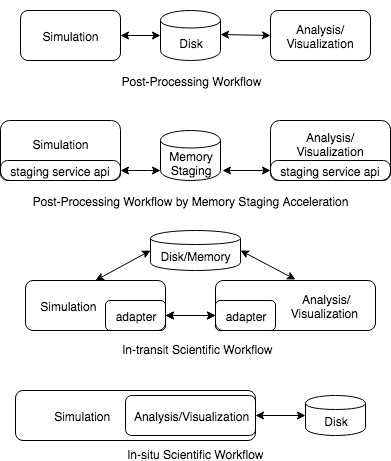
\includegraphics[width=0.75\linewidth]{./figure/scientificworkflowpattern.jpg}
\caption{Scientific Workflow Pattern}
 \label{fg:state}
\end{figure} 


The main task of scientific workflow aims to solve the problems of how and when to run the task in an automatic way as far as possible. Post-processing can be supported well by workflow based DAG (Directed Acyclic Graph) with fixed dependency before workflow run. Even though there are all kinds of work focusing on the intermediate component such as data staging service or in-situ adaptor to leverage specific scenarios (we will discuss this in Background and related work) there are few works explore how to support hybrid pattern in portable, flexible and scalable way(the aim of the experiments). For example, we could use the in-situ part in the simulation to identify if some interesting things happen, if the interesting happens, the in-transit pattern can be used to notify analysis, analysis and visualization component to load data from staging service can be triggered at the same time. 

One challenge for scientific workflow is how to support the complex integration of application patterns including in-situ, in-transit and post-processing tasks\cite{oldfield2014evaluation}. There are two questions needed to be solved in this scenario. (1) Tasks in a workflow is not in same abstraction level, for example, the in-situ part can be a thread in a program and the post-processing part is another program (2) When to run task is unknown before workflow start, the task could be triggered several times or even not be triggered based on the content of intermediate data application.

Our work provides a method based on event programming to leverage the hybrid scientific pattern including in-situ and in-transit pattern, we also implement an event driving workflow tool to compose the scientific application and evaluate its effectiveness in experiment part. The main advantages of this event-driven workflow include:

(1)The dependency could be defined in a more flexible form based on execution sequence or content of intermediate data.

(2)The workflow tool could help the user to express the dependency and control for tasks with different abstraction level and running pattern such as in-situ, in-transit and post-processing.

(3)There is also potential to combine this workflow with low-level resource scheduler system to leverage whole running task of the scientific workflow (more detailed after experiments finishing, maybe provide some good practice to implement the hybrid workflow including in-situ in-transit and post-processing)

The rest paper is organized as follows, Section \uppercase\expandafter{\romannumeral2} introduce the background and the related work of event-driven workflow, Section \uppercase\expandafter{\romannumeral3} introduce the design and implementation of workflow framework. Section \uppercase\expandafter{\romannumeral4} presents the experiments to show the performance and effectiveness of the framework. Section \uppercase\expandafter{\romannumeral5} introduce the conclusion and the future work of the work.


\section{Background and Related Work}
In this section, we briefly introduce the relevant work of scientific application from the aspect of task dependencies, then we introduce the workflow system that supports those using scenarios and explain the shortage of current workflow system, at last, we will introduce the pub-sub mechanism and it's using in the workflow system.

\subsection{Types of Scientific Application and Workflow System}
Considering the scientific application in \cite{makeflowexample}, the execution of tasks in workflow could be represented as DAG (Directed Acyclic Graph), every node represent the execution of the task and every edge represent the sequence of the execution between tasks. For workflow tool such as \cite{makeflowexample,wilde2011swift}, the abstraction of DAG should be fixed before the application running, the user should grasp the topology of the task dependency in advance and execute the workflow by submitting the description file, then workflow will schedule and execute the task according to this DAG blueprint. The intermediate file was used to control the execution of the typical dependency pattern\cite{bharathi2008characterization}.

There are other types applications without fixed and explicit task dependency pattern before the task running, the task may or may not be triggered during task running and it depends on the content of the data instead of the input/output data files in those cases. For example, in simulation-analyzing-visualization workflow, a large amount of simulation data will be generated in short time, some simulation will also running several days, there are some redundant data in the output of the data but only some of them are useful data. If we only want to visualize the data with the average value larger than the specific threshold, the picture will be plotted only when data satisfy our predefined condition. There are several strategies for workflow system to address this issue, one is post-processing which will load all the simulation data into the disk and then process the data in separate tasks. But this solution only useful for small-scale simulation, the increasing data, size and limited storage and bandwidth make high fidelity post-processing impractical\cite{ayachit2015paraview}. In situ workflow is the latest trend to solve this issue\cite{dreher2017situ}. There are several intermediate components to leverage the in-situ workflow\cite{docan2012dataspaces,ayachit2015paraview}  there are works exploring how to decompose original algorithm into in-situ method such as\cite{bennett2012combining} some works are exploring the properties of workflow at exascale\cite{dreher2017situ} but few works focusing on how workflow support different type of in-situ tasks involving flexible dependencies relationship. 

\subsection{Types of Dependencies between Workflow Tasks}
One critical distinction between the traditional workflow(without in-situ task) and the in-situ workflow is the construction of task dependencies. For traditional workflow such as \cite{albrecht2012makeflow}, the dependencies are determined by input and output files between tasks, for example, if the output file of task A is the input of task B there is a dependency between task A and task B namely task B needed to be started after taskA finish.  In the in-situ/in-transit/Hybrid workflow, the dependency will be described in much finer granularity and more flexible way.  For example, task B will start after one loop iteration of taskA finish, or taskB needed to be started when the output of taskA satisfy the specific condition. According to the Figure 1 in the introduction, this is a kind of hybrid pattern: the in-situ part will be used to detect if the interested happens and then the in-transit pattern will be triggered to analyze the data. Dedicated communication libraries needed to be used to send the message between different tasks to synchronize the execution of the task, namely to decide when the task is supposed to be started. No matter for the traditional task or in situ tasks, the task dependency pattern could be divided into three main types \cite{albrecht2012makeflow,bharathi2008characterization} which are shown in Figure 2. 
\begin{figure*} 
\centering
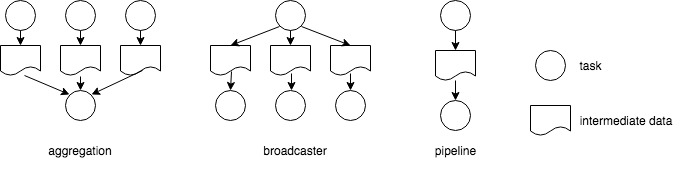
\includegraphics[width=.8\linewidth]{./figure/taskpattern.jpg}
\caption{typical workflow pattern}
 \label{fg:state}
\end{figure*} 

For traditional workflow, the intermediate data are files on the disk and the work queue\cite{albrecht2012makeflow} could be used to control the execution of tasks,  for in-situ workflow, one solution is to view the intermediate data as series of event messages which will be used to control the task execution sequence generated by in-situ tasks or infrastructure running the tasks.

\subsection{Pub-Sub paradigm and event-driven workflow pattern}

Once we assume event message as a special intermediate data used to synchronize the task execution, Pub-Sub paradigm \cite{eugster2003many} could satisfy the requirements to run fine granularity task dependency by messaging communication in the distributed way, There are also all kinds of implementation in research and industry using event message broker based on those pub-sub-notify architecture\cite{hivemq,jin2012scalable,redispubsub}, but there are few scientific workflow systems combining the task dependency and event driving programming together. Some works such as \cite{jin2012scalable} use this mechanism to leverage the in situ workflow, but they only support the specific underlying library and the types of task dependency pattern is also limited. A canonical pub-sub mechanism works in three steps , assume there are two component namely subscriber $S$ and publisher $P$ (1) $S$ will subscribe one or more interesting events into the pub-sub broker (2) $P$ will push events into the pub-sub broker (3)  pub-sub broker will notify $S$ if pushed event match the subscribed event. There exists a dependency between publisher and subscriber in this paradigm. If we use this programming model to compose workflow, the task could be a publisher or subscriber at in the workflow, there will be less restriction on task because any type of tasks could generate the event used to construct the dependency , the task can be in-situ part of the task or jobs running by sbatch system flexibly according to different using scenarios. By this task composing model,  This kind of event-driven workflow should support the task paradigm in Figure 3.
\begin{figure*} 
\centering
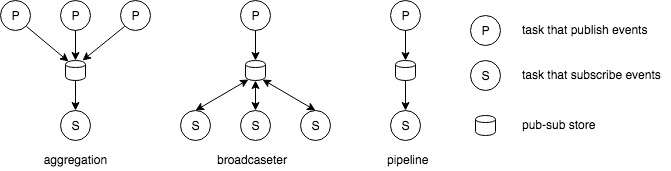
\includegraphics[width=.8\linewidth]{./figure/edtaskpattern.jpg}
\caption{typical event-driven workflow pattern}
 \label{fg:state}
\end{figure*} 
One advantage to use event message to express dependency is the flexibility for dependency granularity, the event message is an abstraction of the user-defined dependent data bock which could be the disk files or data instance in memory. 
There are following scenarios to use event programming to leverage scientific workflow:

(1)Event messages could also represent the properties of data and runtime, for example, an event could represent data in a specific domain is larger than a threshold

(2)The status of underlying infrastructure, the start, stop of runtime system(batch runtime system or container runtime system)

(3)In-situ, in-transit and post-processing tasks can be composed together in a workflow by event message abstraction

The broadcaster and pipeline pattern are supported by pub-sub-notify mechanism naively but there is no support for aggregation pattern. For typical pub-sub mechanism, is subscriber subscribe multiple events such as eventA, eventB eventC, and publishing of those three events will notify the subscriber and trigger execution of task, however, in workflow aggregation scenario, the specific subscribed runtime is supposed to be triggered when all eventA , eventB and eventC are published and satisfied. We will discuss the details of pub-sub event store and relevant runtime client to support all of those patterns in implementation part. 



\section{Implementation}
We introduce the architecture of event-based workflow system and then discussed the details for every component. Figure 3 shows the architecture of event-driven workflow and it's work procedure.

\begin{figure} 
\centering
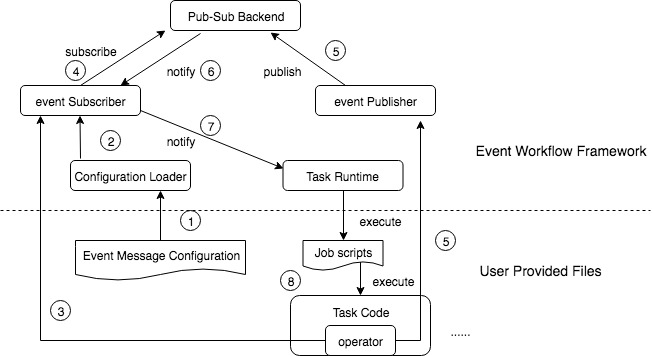
\includegraphics[width=1\linewidth]{./figure/edflowarchitecture.jpg}
\caption{Event driven workflow framework archetecture}
 \label{fg:state}
\end{figure} 


The user view and the workflow frame view are shown in Figure 3,  User needs to provide the initial configuration files which include the path of the job script and the event that every task interested, those events will be subscribed into the event store. The operator is the in-situ part integrated into the simulation code which is used to send subscribe and publish request during the simulation run. When specific events are published, the subscribing end will be notified and the job scripts will be started by task runtime. Several typical and in-situ using scenarios can be supported because this event pub-sub backend support pub-sub in 1:1, 1:n and n:1 manner and a user-defined event also provide flexibility to express the task dependency in fine-grained ways. 

(1) Traditional predefined static dependency tasks can be supported by running operator before task start running (subscribe event) after the task finish (publish event), the task will start running only when the specific event happens.

(2) The granularity of data dependency can be defined by the user in a flexible way to avoid post-processing and decrease all the workflow running time. For example, when every thread generates specific domain data, the visualization task can be notified and triggered immediately when all the subscribed events are satisfied.

More detailed using scenarios will be discussed in experiments and evaluation. We will introduce the key component for the following parts. 

\subsection{Optimised Pub-Sub Backend}

In this part, we introduce the design and implementation of optimized pub-sub mechanism and discuss how it supports both traditional and in-situ task dependency pattern in a workflow. Besides, we also leverage the canonical pub-sub mechanism and make it support the aggregation(fan-in) and broadcaster(fan-out) pattern at the same time, namely one event subscriber could subscribe multiple sub-event messages and specify the triggering conditions, when all the events are published specific times, the subscribed events will be triggered subsequently. The simplified underlying data structure is shown in Figure 6, eventually, we need to maintain several core maps to keep the mapping relation from one client id to several subscribed events and from one event to several client ID that interested to it. besides, we also need to use another map to record the published times for every event and use this info to check if the specific client should be notified. the subscribe and publish method is described as follows:

(1) event subscribe: For every subscribe request, there is a new id will be unique id will be generated and stored at back end, the event that this client interested will also be recorded and associated map will be initialised, there is a house-keeping logic in every subscribe method keeps checking the satisfactory flag, request will block here if the flag is not satisfied, otherwise the notify status will be returned back to client.

(2) event publish: When there is publish request, the backend will parse the event message in a request and retrieve the event from the map of an event to subscribe client id. For example, if we assume the publishing event is EVENTA. For every client id, we could get the event set it subscribed(every client is associated with an event message set), we could find EVENTA from this set and increase one for the number it is pushed, then we could check the required triggering number in published event, if the number equals to the required number, we could set the satisfied flag as true.

\subsection{Event Configuration and Data Operator}


\subsection{Task Runtime}
Task Runtime is designed to support multiple drivers to execute a task. The input of the task runtime is the driver name and the path of the running scripts. If the driver is the container solution such as Singularity or Docker, the execution path could be the name of the image.



\section{Evaluation and Experiments}
We have evaluated the performance of the event driven workflow tool on Caliburan cluster at Rutgers Discovery Informatics Institute. The Caliburan cluster is based on a FatTwin SuperServer system. It has 560 nodes, each with two Intel Xeon E5-2695 v4 (Broadwell) processors, 256 gigabytes (GB) of RAM, and a 400 GB Intel NVMe drive. Overall, the system has 20,160 cores, 140 TB of memory and 218 TB of non-volatile memory. The performance is 603 TFLOPS with a peak performance of 677 TFLOPS\cite{caliburn}.

\subsection{Performance Evaluation}
The first experiment is measure the latency of task triggering time. The test using synthetic workflow include two tasks, taskB depends on taskA. Our test based on the workflow pattern in Figure 2 which include aggregation, broad caster and chained pattern. For every latency, we also compare our workflow tool with the other workflow tool Swift\cite{wilde2011swift} and Makeflow\cite{albrecht2012makeflow}.

For chained pattern when taskA.X finish taskB.X will be triggered, we increase the number of coupling pairs of (taskA.X, taskB.X) to test the latency.

For aggregation pattern, there are several taskA.X and one taskB, when all taskA.X finished, task.B will be triggered and we will test waiting time of the taskB with the increasing number of taskA.X

For broadcaster pattern, there are one taskB and several taskA.X, when taskA finish, all the task.B will be triggered and we will test the average waiting time of the taskB with the increasing of the taskB.X.

\subsection{hybrid workflow using scenarios}
In this part, we use a real use case to show how event workflow tool compose different abstraction of task and leverage the scientific application.
Figure ? shows the different between the traditional post-processing workflow and the hybrid event driven workflow. We could notice that in-situ task and the post-processing task could be composed together by event driven workflow and the synchronization between different task is also minimized by event messages.

\begin{figure} 
\centering
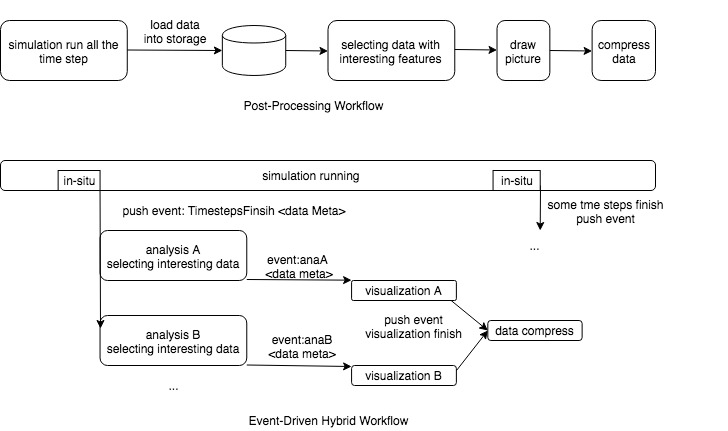
\includegraphics[width=1.0\linewidth]{./figure/hybridapplication.jpg}
\caption{Scientific Workflow Pattern}
 \label{fg:state}
\end{figure} 

\section{Conclusion}

support more types of task running tool

Future work: the language/compiler tool to facilitate the creation of the event configuration

make pub/sub in more scalable level and let it more distributed

challenge, traditional dependency is in layered way but new pattern is in flattern way

more suitable for the task with run in several time and specific things will happen for several times. not cascade pattern


% trigger a \newpage just before the given reference
% number - used to balance the columns on the last page
% adjust value as needed - may need to be readjusted if
% the document is modified later
%\IEEEtriggeratref{8}
% The "triggered" command can be changed if desired:
%\IEEEtriggercmd{\enlargethispage{-5in}}

% references section

% can use a bibliography generated by BibTeX as a .bbl file
% BibTeX documentation can be easily obtained at:
% http://www.ctan.org/tex-archive/biblio/bibtex/contrib/doc/
% The IEEEtran BibTeX style support page is at:
% http://www.michaelshell.org/tex/ieeetran/bibtex/
%\bibliographystyle{IEEEtran}
% argument is your BibTeX string definitions and bibliography database(s)
%\bibliography{IEEEabrv,../bib/paper}
%
% <OR> manually copy in the resultant .bbl file
% set second argument of \begin to the number of references
% (used to reserve space for the reference number labels box)

\bibliographystyle{plain}
\bibliography{reference}

% that's all folks
\end{document}


